\documentclass[12pt]{article}
\usepackage[a4paper,left=1.18in,right=0.59in,top=1.33in,bottom=1.46in,includefoot]{geometry}
\usepackage{fontspec}
\setmainfont{Times New Roman}
\usepackage{setspace}
\usepackage{hyperref}
\usepackage{enumitem}
\usepackage{tikz}
\usepackage{longtable}
\usepackage{booktabs}
\usepackage{array}
\usepackage[normalem]{ulem}
\usepackage{caption}
\usepackage{amsmath}
\usepackage{amssymb}
\hypersetup{hidelinks}
\setstretch{1.58}
\setlength{\parindent}{0pt}
\setlength{\parskip}{0.03\baselineskip}
\setlist[itemize]{leftmargin=2.2em,labelsep=0.55em,itemsep=0.08\baselineskip,topsep=0.1\baselineskip,parsep=0pt}
\setlist[enumerate]{leftmargin=2.4em,labelsep=0.55em,itemsep=0.08\baselineskip,topsep=0.1\baselineskip,parsep=0pt}
\setcounter{secnumdepth}{0}
\newcommand{\proposalSubheading}[1]{%
  \par\addvspace{0.38\baselineskip}%
  \noindent\textbf{#1}\par\nobreak\addvspace{0.08\baselineskip}%
}
\newcommand{\proposalResultHeading}[1]{%
  \par\addvspace{0.45\baselineskip}%
  \noindent\textbf{#1}\par\nobreak\addvspace{0.06\baselineskip}%
}
\newcommand{\TOCentry}[3]{%
  \noindent\hyperref[#3]{\makebox[2.4em][l]{#1}#2}\nobreak\dotfill\ \hyperref[#3]{\pageref*{#3}}\par\vspace{0.15em}%
}
\begin{document}

\begin{titlepage}
\newgeometry{left=1.18in,right=0.59in,top=1.33in,bottom=0.7in}
\centering
\vspace*{0.4cm}
{\Large\bfseries INTEGRATING ERC-20 ALLOWANCE EDGES INTO PAGERANK FOR ENHANCED ON-CHAIN WALLET REPUTATION SCORING\par}
\vfill
{by\par}
\vspace{0.7cm}
{\large\bfseries TAEHONG KWON\par}
\vfill
{submitted in accordance with the requirements for the degree of\par}
\vspace{0.7cm}
{\large\bfseries DOCTOR OF PHILOSOPHY\par}
\vspace{0.35cm}
{in the subject\par}
\vspace{0.7cm}
{\large\bfseries COMPUTER SCIENCE\par}
\vfill
{at the\par}
\vspace{0.7cm}
{\large\bfseries UNIVERSITY OF SOUTH AFRICA\par}
\vfill
{SUPERVISOR: Prof. Ernest Mnkandla\par}
\vspace{0.35cm}
{CO-SUPERVISOR: Prof. Donatien Koulla Moulla\par}
\vfill
{June 2025\par}
\end{titlepage}
\restoregeometry

\phantomsection
\section*{Abstract}
\label{sec:abstract}

The financial system has generated broad-based growth impetus by allocating capital efficiently through lending. In this light, the advancement of DeFi is likewise expected to hinge critically on the degree of on-chain lending activity. However, DeFi platforms face constraints in executing collateral-backed loans due to difficulties in enforcing collateral assets, and they similarly confront limitations in offering unsecured credit, since traditional credit-scoring models that incorporate tangible-asset and employment information cannot be applied directly.


Existing PageRank-based methods, such as the Adaptive Weighted PageRank (AWP) algorithm, primarily rely on transaction volume and recency (time-decay) to assess wallet trustworthiness. While these approaches effectively capture eco- nomic flows and activity levels, they might incur substantial computational overhead by requiring exhaustive parsing of historical transactions.


This study proposes EndorseRank, a novel on-chain reputation metric leveraging ERC-20 approve and permit allowances as direct indicators of wallet endorsement. Each approve/permit action explicitly grants spending permissions to another wallet, inherently representing trust. By constructing a directed, weighted graph $G_{\text{approve}}$based solely on the most recent allowance amounts for each wallet pair, EndorseRank eliminates the need for historical time-decay adjustments and significantly reduces computational complexity.


The proposed EndorseRank algorithm utilizes PageRank methodology on this allowance-based graph. Our research aims to:


\begin{enumerate}
\item[1.] Develop a robust data pipeline to extract and manage the latest approve/permit allowances.
\item[2.] Construct and efficiently compute reputation scores from a sparse and endorsement- oriented graph.
\item[3.] Evaluate EndorseRank's predictive accuracy concerning on-chain financial risk (e.g., defaults on Aave) compared to established transaction-based methods, using metrics such as AUC, precision, and recall.
\item[4.] Conduct extensive computational benchmarks to demonstrate superior efficiency in runtime and memory usage.
\end{enumerate}
By addressing these objectives, EndorseRank seeks to provide a computation- ally efficient, semantically clear, and accurate reputation scoring mechanism suitable for real-world DeFi platforms, enabling better risk management and decision- making.


\textbf{\emph{Keywords--- }}\textbf{DeFi, On-Chain Reputation, On-Chain Financial Risk Prediction, Blockchain Data Analytics, Predictive Modeling, Wallet Endorsement Graph}


\clearpage
{\Large\bfseries Table of Contents\par}
\vspace{0.75em}
\TOCentry{1}{{\textbf{Introduction and background}}}{sec:introduction-and-background}
\TOCentry{2}{{\textbf{Research Problem}}}{sec:research-problem}
\hspace*{1.5em}\TOCentry{2.1}{{Research Questions}}{sec:research-questions}
\hspace*{1.5em}\TOCentry{2.2}{{Objectives}}{sec:objectives}
\hspace*{1.5em}\TOCentry{2.3}{{Expected Results}}{sec:expected-results}
\TOCentry{3}{{\textbf{Literature Review}}}{sec:literature-review}
\hspace*{1.5em}\TOCentry{3.1}{{Graph-Based On-Chain Reputation Scoring}}{sec:graph-based-on-chain-reputation-scoring}
\hspace*{1.5em}\TOCentry{3.2}{{Predictive Modeling for On-Chain Credit Risk}}{sec:predictive-modeling-for-on-chain-credit-risk}
\hspace*{1.5em}\TOCentry{3.3}{{Industry Initiatives and Non-Scholarly Perspectives}}{sec:industry-initiatives-and-non-scholarly-perspectives}
\TOCentry{4}{{\textbf{Theoretical Framework}}}{sec:theoretical-framework}
\hspace*{1.5em}\TOCentry{4.1}{{Constructs and Variable Mapping}}{sec:constructs-and-variable-mapping}
\hspace*{1.5em}\TOCentry{4.2}{{Conceptual Model}}{sec:conceptual-model}
\hspace*{1.5em}\TOCentry{4.3}{{Theoretical Justification}}{sec:theoretical-justification}
\hspace*{1.5em}\TOCentry{4.4}{{Implications for Research Design}}{sec:implications-for-research-design}
\TOCentry{5}{{\textbf{Research Methodology}}}{sec:research-methodology}
\hspace*{1.5em}\TOCentry{5.1}{{Research Design and Method}}{sec:research-design-and-method}
\hspace*{1.5em}\TOCentry{5.2}{{Data Analysis}}{sec:data-analysis}
\TOCentry{6}{{\textbf{Limitations}}}{sec:limitations}
\TOCentry{7}{{\textbf{Ethics Considerations}}}{sec:ethics-considerations}
\TOCentry{8}{{\textbf{Significance of Research}}}{sec:significance-of-research}
\TOCentry{9}{{\textbf{Schedule}}}{sec:schedule}
\TOCentry{10}{{\textbf{Dissertation/Thesis Outline}}}{sec:dissertationthesis-outline}
\hspace*{1.5em}\TOCentry{10.1}{{Data Analysis}}{sec:dissertationthesis-outline}
\TOCentry{11}{{\textbf{Appendices}}}{sec:appendices}
\clearpage

\clearpage
\phantomsection
\section*{1 \textbf{Introduction and background}}
\label{sec:introduction-and-background}
\addcontentsline{toc}{section}{1 Introduction and background}

Decentralized Finance (DeFi) has expanded lending and borrowing activity on public blockchains, yet most lending remains highly collateralized because protocols cannot rely on traditional off-chain identity, employment, or credit histories. In a pseudonymous setting, the core challenge is not merely allocating capital, but allocating it safely: identifying which wallets are likely to behave reliably in credit-like interactions (e.g., repeated borrowing, repayment, and delegation of spending rights), while limiting exposure to opportunistic or malicious actors (e.g., defaulting, griefing, Sybil-style account creation, and rapid reputation farming).


In this study, on-chain wallet reputation scoring refers to the process of computing a quantitative score for a blockchain address using observable on-chain behavior and relationships, with the goal of approximating trustworthiness or credit-related reliability without relying on off-chain personal data. In DeFi, such scores can support (i) more accurate assessment of on-chain financial risk(e.g., default or liquidation events), (ii) improved risk controls for lending protocols, and (iii) potential pathways toward more capital-efficient credit (e.g., reduced collateral requirements for low-risk participants).


To avoid ambiguity, the key concepts used throughout this proposal are defined as follows:


\begin{itemize}
\item[\textbullet] \textbf{DeFi (Decentralized Finance): }Financial services (e.g., lending, borrowing, exchanges) implemented via smart contracts on public blockchains.
\item[\textbullet] \textbf{Wallet / Address: }A blockchain account that can hold assets and interact with smart contracts (used as the unit of analysis).
\item[\textbullet] \textbf{On-chain reputation / reputation score: }A numerical indicator computed from on-chain signals intended to represent a wallet's reliability in financial interactions.
\item[\textbullet] \textbf{On-chain credit risk / default event: }Observable adverse outcomes such as loan default, liquidation, or protocol-defined delinquency signals.
\item[\textbullet] \textbf{PageRank / Weighted PageRank: }Graph-based ranking methods that propagate influence through directed edges, optionally weighted by edge strength.
\item[\textbullet] \textbf{ERC-20 allowance: }A state variable recording how much a token owner permits a spender to transfer on the owner's behalf.
\item[\textbullet] \textbf{Approve / Permit: }ERC-20 mechanisms that set allowances; permit (e.g., EIP-2612-style) enables allowance updates via signed messages.
\item[\textbullet] \textbf{Endorsement graph: }A directed graph where an edge represents an explicit delegation/endorsement signal rather than a mere transfer.
\end{itemize}
Reputation scoring is critical in credit-based lending to distinguish reliable participants from potential bad actors. Recent examples of on-chain wallet reputation scoring inspired by PageRank include the AWP algorithm proposed by Do et al. (2023), which assigns reputation scores based on transaction volume (greater inflows imply greater trust) and activeness (recent transactions receive higher weight via a logistic time-decay function). While this approach captures both economic magnitude and temporal relevance, it does not directly model explicit spending authorization as a trust signal.


The ERC-20 token standard, however, includes two explicit allowance mechanisms---approve and permit---by which a token holder grants another address per- mission to spend up to a specified amount on its behalf. Each approval event inherently represents an endorsement, where the approved amount directly quantifies the granularity of trust. By extracting only the latest allowance for each owner \(\to\) spender pair, we can build a directed, weighted endorsement graph $G_{\text{approve}}$, in which each edge's weight equals the most recent approved token amount. This de- sign eliminates the need for any time-based decay---since newer approvals override older ones---and focuses computation on the most salient, up-to-date trust signals.


Clarifying the importance in DeFi, enhancing on-chain wallet reputation scoring can provide concrete benefits:


\begin{itemize}
\item[\textbullet] \textbf{Risk management and protocol safety: }Better identification of risky wallets can reduce bad debt and improve the stability of lending markets.
\item[\textbullet] \textbf{Capital efficiency: }More informative trust signals can support differentiated risk parameters (e.g., borrowing limits or collateral requirements) instead of one-size-fits-all constraints.
\item[\textbullet] \textbf{Access and inclusion without off-chain data: }On-chain scoring can enable participation for users who lack conventional credit records, while preserving the DeFi principle of permissionless access.
\item[\textbullet] \textbf{Composable trust for DeFi applications: }A reusable reputation layer can be consumed by multiple protocols (e.g., lenders, insurers, and DAOs) to make consistent, explainable decisions.
\end{itemize}
Despite the clear endorsement semantics and sparser graph structure of approval-based relationships, no existing study has systematically leveraged ERC-20 allowances as primary edge weights for PageRank. This methodological gap motivates EndorseRank, our proposed on-chain reputation algorithm that applies to a standard Weighted PageRank to $G_{\text{approve}}$. We hypothesize that EndorseRank will achieve comparable or superior predictive power for financial risk (e.g., default events) while significantly reducing data-processing complexity compared to transaction- value-- and time-decay--based methods. To ensure a clear alignment between this motivation and what the study will deliver, the proposal specifies objective-linked expected results:


\begin{itemize}
\item[\textbullet] A reproducible pipeline and latest-allowance endorsement graph derived from ERC-20 approve/permit states;
\item[\textbullet] An optimized, scalable Weighted PageRank implementation (EndorseRank) operating on this sparse, trust-semantic graph; and
\item[\textbullet] Empirical evidence using transactions of the DeFi lending platform such as Aave and standard metrics that EndorseRank matches or improves risk-prediction performance relative to transaction-based baselines while reducing computational overhead.
\end{itemize}
\clearpage
\phantomsection
\section*{2 \textbf{Research Problem}}
\label{sec:research-problem}
\addcontentsline{toc}{section}{2 Research Problem}

Current on-chain reputation methods using PageRank rely primarily on transaction values to infer economic ties among wallets. While AWP algorithm has shown promise (Do et al., 2023), it exposes two practical limitations when used as a general-purpose on-chain reputation signal. First, reproducing transaction-based PageRank at Ethereum scale typically requires exhaustive parsing and aggregation of historical transfers, which increases data-processing cost, memory footprint, and iteration time for convergence. This computational burden becomes especially problematic when reputation is intended to be computed repeatedly or near real-time for DeFi risk monitoring.


Second, transaction value is an indirect and sometimes ambiguous proxy for "trust." Wallets may exchange tokens for many reasons (e.g., trading, arbitrage, airdrops, or automated contract activity) without expressing endorsement or delegating spending authority. Yet delegated permission is central to credit exposure in DeFi lending and risk assessment (Wolf et al., 2022; Ghosh et al., 2024). By contrast, the ERC-20 allowance mechanism explicitly encodes delegation through approval (and, where supported, permit) updates that authorize a spender to transfer tokens on an owner's behalf (EIP-20; EIP-2612). Because an approval remains in force until changed, the latest allowance state between each owner--spender pair offers a direct, current endorsement signal that can be represented as a sparse directed graph, aligning with network-propagation style risk scoring used in related graph-based models (Imig, 2023; Yang et al., 2024).


Thus, the central research problem is: Can we construct an on-chain wallet reputation metric using ERC-20 approve/permit relationships that reduces computational cost, more faithfully represents endorsement semantics, and yields equal or superior predictive accuracy for financial risk (e.g., default events) compared to transaction-based PageRank methods?


To address this issue, we will design, implement, and evaluate the EndorseRank algorithm, which constructs a sparse, directed, weighted endorsement graph using ERC-20 approve and permit calls. The key challenges include accurately extracting the most recent approve/permit states between each owner--spender pair so that outdated allowances do not distort the graph; ensuring rapid convergence of the PageRank algorithm on large but sparse endorsement graphs; and evaluating how effectively EndorseRank correlates with observable credit risk outcomes such as default or liquidation events in lending protocols (e.g., Aave) (Wolf et al., 2022).


\phantomsection
\subsection*{2.1 Research Questions}
\label{sec:research-questions}
\addcontentsline{toc}{subsection}{2.1 Research Questions}

In the setting of Ethereum-based DeFi lending, from the perspective of DeFi protocols, risk analysts, wallet users, and researchers who need explainable wallet-level risk indicators, can EndorseRank---a Weighted PageRank metric built from ERC-20 approval/permit-derived allowance relationships---match or outperform Adaptive Weighted PageRank and transfer-based PageRank baselines, as measured by rank divergence, default/liquidation prediction performance, runtime, memory use, and convergence stability?


\begin{longtable}{>{\raggedright\arraybackslash}p{0.27\linewidth}>{\raggedright\arraybackslash}p{0.66\linewidth}}
\caption{SPICE framework for the main research question}\\
\toprule
\textbf{SPICE Element} & Description \\
\midrule
\textbf{Setting} & Ethereum-based DeFi lending and on-chain wallet reputation scoring \\
\addlinespace
\textbf{Perspective} & DeFi protocols, risk analysts, wallet users, and researchers who need explainable wallet-level risk indicators \\
\addlinespace
\textbf{Intervention} & EndorseRank, a Weighted PageRank metric built from ERC-20 approval/permit-derived allowance relationships \\
\addlinespace
\textbf{Comparison} & Adaptive Weighted PageRank and transfer-based PageRank models that rely on historical transaction flows \\
\addlinespace
\textbf{Evaluation} & Rank divergence, default/liquidation prediction performance, runtime, memory use, and convergence stability \\
\addlinespace
\bottomrule
\end{longtable}

\proposalSubheading{• Graph Construction and Fidelity}

\begin{itemize}
\item[\textendash] RQ1.1: How can we preprocess ERC-20 approve and permit events to construct a reliable, up-to-date weighted endorsement graph that reflects current token allowances?
\item[\textendash] RQ1.2: Does a graph based on approve/permit edges preserve a sufficient trust signal compared to transaction-value graphs?
\end{itemize}
\proposalSubheading{• Ranking Comparison}

\begin{itemize}
\item[\textendash] RQ2.1: How does EndorseRank's ranking output differ from AWP and traditional transaction-based PageRank scoring in terms of relative ordering of wallets?
\item[\textendash] RQ2.2: To what extent do EndorseRank scores correlate with AWP scores, and where do they diverge?
\end{itemize}
\proposalSubheading{• Risk Prediction and Interpretability}

\begin{itemize}
\item[\textendash] RQ3.1: What is the statistical correlation between EndorseRank scores and on-chain default or liquidation events (e.g., on Aave V3)?
\item[\textendash] RQ3.2: How does EndorseRank's predictive power (e.g., measured via AUC, precision, recall) for default events compare to that of AWP and transaction-based PageRank?
\end{itemize}
\proposalSubheading{• Computational Efficiency}

\begin{itemize}
\item[\textendash] RQ4.1: What is the execution time and resource usage (CPU, memory) required to compute EndorseRank versus AWP for a fixed set of wallets?
\item[\textendash] RQ4.2: How does graph sparsity (approve/permit vs. transfer edges) affect convergence speed and floating-point stability in PageRank iterations?
\end{itemize}
\phantomsection
\subsection*{2.2 Objectives}
\label{sec:objectives}
\addcontentsline{toc}{subsection}{2.2 Objectives}

The overarching goal of this study is to design, implement, and evaluate an EndorseRank algorithm that leverages ERC-20 approve/permit allowances as edge weights without any time decay factors---to produce a computationally efficient and trust- reflective on-chain reputation score. Specifically, we aim to:


\proposalSubheading{1. Graph Construction}

\begin{itemize}
\item[\textbullet] \textbf{O1.1: }Build a data-extraction pipeline that scans the Ethereum blockchain for ERC-20 \textbf{Approve }and \textbf{Permit }events, isolates the most recent allowance amount for each owner \(\to\) spender pair, and stores these values.
\begin{itemize}
\item[\textendash] \emph{Rationale: }Since each new approve/permit transaction overrides previous allowances for the same owner \(\to\) spender, only the latest allowance per pair needs to be retained.
\end{itemize}
\item[\textbullet] \textbf{O1.2: }Construct a directed, weighted graph $G_{\text{approve}}$in which each node represents an ERC-20 wallet, and each edge (u\(\to\)v) carries a weight equal to the \textbf{latest allowance amount }(e.g., in ETH or token units) from wallet u (owner) to wallet v (spender).
\begin{itemize}
\item[\textendash] \emph{Detail: }We do \textbf{not }apply any time-based decay or history aggregation; all older approvals are superseded by the most recent event.
\end{itemize}
\end{itemize}
\proposalSubheading{2. EndorseRank Algorithm Implementation}

\begin{itemize}
\item[\textbullet] \textbf{O2.1: }Implement a \textbf{Weighted PageRank }algorithm on $G_{\text{approve}}$, where each node's ``score'' is computed by distributing its PageRank mass to outgoing edges proportionally to the allowance weights.
\begin{itemize}
\item[\textendash] \emph{Specifications:}
\begin{enumerate}
\item[(a)] Normalize each node's outgoing edges so that for node u, the probability of transitioning to neighbor v is:
\end{enumerate}
\end{itemize}
\end{itemize}
\[P_{u\to v} = \frac{w_{u\to v}}{\sum _{x\in N^{+}(u)}w_{u\to x}}\]

where N\textsuperscript{+}(u) is the set of out-neighbors of u (all nodes x that u approves), x is an element of N\textsuperscript{+}(u), and $W_{u\to v}$is the latest allowance amount from wallet u to wallet v.


\begin{enumerate}
\item[(b)] The equation above specifies the transition probability used by EndorseRank: $P_{u\to v}$ equals Wu\(\to\)v divided by the sum of all outgoing allowance amounts from wallet u, where each $W_{u\to v}$ denotes the latest allowance amount on edge u\(\to\)v. Thus, each wallet distributes its PageRank mass only across currently active approval relationships, proportionally to normalized allowance strength.
\item[(c)] Use a standard damping factor (e.g., 0.85), but do not incorporate any additional time-weighting or value-decay beyond the raw allowance. This keeps the transition model consistent with PageRank-style convergence guarantees, avoids tuning extra hyperparameters without empirical justification, and preserves comparability to baselines that are defined over raw allowance weights rather than time-adjusted scores.
\end{enumerate}
\begin{itemize}
\item[\textbullet] \textbf{O2.2: }Optimize the EndorseRank implementation for large, sparse graphs by using sparse-matrix representations and efficient iterative solvers, ensuring that convergence is achieved with minimal memory overhead and fast runtime.
\end{itemize}
\proposalSubheading{3. Reproduction of Baselines and Data Consistency}

\begin{itemize}
\item[\textbullet] \textbf{O3.1: }Reproduce two baseline ranking approaches on an identical wallet set drawn from the Aave V3 credit-lending ecosystem over the same time window:
\end{itemize}
\begin{enumerate}
\item[(a)] Adaptive Weighted PageRank (AWP): a transaction-value--weighted PageRank that applies time-decay factors to transfers.
\item[(b)] Transfer-Based Weighted PageRank: a simpler model that uses raw ERC-20 transfer amounts as edge weights, without time decay.
\end{enumerate}
\begin{itemize}
\item[\textbullet] \textbf{O3.2: }Maintain a uniform data-processing pipeline so that EndorseRank, AWP, and Transfer-Based PageRank all operate on the same set of wallets and the same period's events, ensuring that any differences in results are due solely to the ranking logic rather than data inconsistencies.
\end{itemize}
\proposalSubheading{4. Performance Evaluation}

\begin{itemize}
\item[\textbullet] \textbf{O4.1: }Compute\textbf{ }Spearman's rho and Kendall's tau between EndorseRank scores and each of the two baselines (AWP and Transfer-Based PageRank) to quantify how similarly or differently wallets are ordered. Spearman's rho captures monotonic rank agreement, while Kendall's tau measures pairwise ordering agreement.
\item[\textbullet] \textbf{O4.2:}\textbf{ }Compare the distribution of scores (e.g., mean, median, interquartile range) for EndorseRank versus the baselines, identifying any outlier wallets that receive disproportionately high approval-based weights but low transfer-based weights (or vice versa).
\item[\textbullet] \textbf{O4.3}: Risk Prediction Performance
\begin{itemize}
\item[\textendash] Label wallets as ``defaulted'' or ``not defaulted'' based on their on- chain liquidation events in Aave V3.
\item[\textendash] Using each ranking score as a predictive feature, train simple classifiers (e.g., logistic regression and random forest) to distinguish defaulted wallets. Logistic regression provides an interpretable linear baseline, while random forest captures nonlinear feature interactions and serves as a robust benchmark for heterogeneous on-chain behavior.
\item[\textendash] Evaluate AUC, precision, recall, F1-score, and calibration for each ranking method, determining whether EndorseRank yields equal or superior predictive accuracy compared to AWP and Transfer-Based PageRank.
\end{itemize}
\end{itemize}
\proposalSubheading{5. Computational Efficiency and Scalability Analysis}

\begin{itemize}
\item[\textbullet] \textbf{O5.1 Runtime Benchmarking: }Measure and compare the total time required (data extraction + graph construction + PageRank convergence) for EndorseRank, AWP, and Transfer-Based PageRank on a fixed wallet set (e.g., 100,000 nodes).
\item[\textbullet] \textbf{O5.2 Memory Profiling: }Record peak memory usage for each method, highlighting how EndorseRank's use of only the latest approval amounts results in a sparser graph and lower memory footprint than transaction- based graphs.
\item[\textbullet] \textbf{O5.3 Convergence Stability}\textbf{: }Analyze the number of iterations needed for each algorithm to reach a predefined convergence tolerance (e.g., 10\textsuperscript{-}\textsuperscript{6}) under different damping factors and token supply scales, verifying that EndorseRank remains numerically stable despite potentially large allowance values.
\end{itemize}
SMART Alignment


The objectives are specific because each one targets a concrete research output: data pipeline, graph construction, algorithm implementation, baseline reproduction, predictive evaluation, and scalability benchmarking. They are measurable through rank-correlation statistics, AUC, precision, recall, F1-score, calibration, runtime, memory, and convergence tolerance. They are attainable and realistic because they use public blockchain logs, Aave V3 liquidation events, reproducible Python-based tooling, and fixed computational resources. They are time-bound through the post-approval schedule, which allocates data extraction, implementation, evaluation, writing, and publication milestones between June 2026 and January 2028.


By accomplishing these objectives, we will demonstrate how a latest-allowance-weighted approach to PageRank can yield a scalable, trust-aligned reputation-scoring model, EndorseRank, that outperforms or matches existing transaction-value-based methods without any time-decay overhead.


\phantomsection
\subsection*{2.3 Expected Results}
\label{sec:expected-results}
\addcontentsline{toc}{subsection}{2.3 Expected Results}

This section states the expected outcomes of the study and explicitly aligns them with the objectives above.


These expected results map directly onto Objectives O1-O5 and mirror the three themes introduced in the background: endorsement-based trust structure, default-risk prediction, and computational efficiency relative to transfer-based baselines.


\proposalResultHeading{ER1: Reproducible allowance dataset and endorsement graph (O1.1-O1.2)}

A documented, reproducible data-extraction pipeline that outputs the latest ERC-20 approve/permit allowance state for each owner-spender pair over a defined time window.


A directed, weighted endorsement graph $G_{\text{approve}}$ constructed from these latest-allowance states, accompanied by summary statistics (e.g., node/edge counts, sparsity, degree distributions) that substantiate the intended sparsity relative to transfer graphs.


\proposalResultHeading{ER2: Scalable EndorseRank implementation (O2.1--O2.2)}

A correct Weighted PageRank implementation that uses latest allowance amounts as edge weights (with a clearly specified damping factor and convergence tolerance) and is optimized for large, sparse graphs.


Evidence of numerical stability under large allowance values and practical convergence behavior (iterations to tolerance) on graphs of increasing size.


\proposalResultHeading{ER3: Baseline reproduction and ranking-difference evidence (O3.1-O4.2)}

Reproduced baseline rankings (AWP and transfer-based weighted PageRank) computed on the same wallet set and the same observation window as EndorseRank.


Quantified agreement and divergence in wallet ordering via Spearman's *\(\rho\)* and Kendall's *\(\tau\)*, alongside targeted case analyses for wallets that are highly ranked by allowance endorsement but not by transfer volume (and vice versa).


\proposalResultHeading{ER4: Risk-prediction results with standard metrics (O4.3)}

A labeled dataset of default/liquidation outcomes (e.g., Aave V3) and comparative evaluation results showing whether EndorseRank yields comparable or superior predictive performance relative to AWP and transfer-based PageRank (AUC, precision, recall, F1, and calibration where applicable).


\proposalResultHeading{ER5: End-to-end efficiency and scalability benchmarks (O5.1-O5.3)}

Runtime and memory profiling results for (data extraction + graph construction + PageRank convergence) demonstrating the computational advantage of using only the latest allowance state versus exhaustive transfer-history parsing.


A scalability analysis that reports how graph sparsity affects convergence speed and resource consumption across methods.


\clearpage
\phantomsection
\section*{3 \textbf{Literature Review}}
\label{sec:literature-review}
\addcontentsline{toc}{section}{3 Literature Review}

\phantomsection
\subsection*{3.1 Graph-Based On-Chain Reputation Scoring}
\label{sec:graph-based-on-chain-reputation-scoring}
\addcontentsline{toc}{subsection}{3.1 Graph-Based On-Chain Reputation Scoring}

Early research on on-chain reputation leveraged graph theory, particularly adaptations of PageRank, to rank wallet addresses by ``trustworthiness.'' Do et al. (2019) provided a first attempt, and subsequent studies formalized this approach for Ethereum. In a recent study, Do et al. (2023) model Ethereum addresses as nodes in a directed graph with transactions as edges, then apply the PageRank algorithm to compute a social credit score for each address. The rationale is that DeFi's growth demands methods to identify and rank entities for unsecured lending and customer protection. In this framework, an address accumulates higher score if it is ``trusted'' by many or large transactions from others, analogous to how important web pages have many incoming links. PageRank thus measures connectivity strength and activity as proxies for reputation. Inspired by the Colendi protocol's vision of a ``social connectivity strength'' metric, these graph models sometimes combine multiple factors (e.g. frequency and volume of interactions) into edge weights. For example, Colendi's system weighted edges by a mix of relation intensity and bilateral activity, feeding into a PageRank-like iterative algorithm to yield a credit score.


A key consideration in graph construction is how to weight the edges. Basic implementations treat each transaction equally, but later work incorporates transaction value as a weight, so that large transfers signify stronger trust. Using a HodgeRank approach, Do et al. (2023) treat the amount of ETH transferred as the weight on each edge and then solve for a global ranking that accounts for these weighted flows. This produces an Ethereum reputation ranking influenced by transaction volume, under the intuition that high-value interactions indicate greater trust or stake between parties. Another practical challenge is dealing with graph structure: Ethereum's transaction graph can contain many isolated clusters or "sink" nodes that absorb PageRank score. Damping factors, as in traditional PageRank, are used to mitigate score inflation for sinks and small isolated subgraphs, ensuring the reputation scores reflect participation in the broader network rather than siloed activity.


One limitation of a vanilla PageRank, i.e., the unmodified PageRank formulation applied to a transaction graph without explicit risk propagation or domain-specific adjustments, is that it may not distinguish malicious but active actors from genuinely reputable ones. Imig (2023) demonstrated that a straightforward PageRank on Ethereum failed to differentiate a known problematic address from a known trustworthy address in terms of score. This highlights the need for refined models. Proposed improvements include incorporating negative feedback or propagation of risk labels through the network. For instance, recent research introduced RiskProp, a network-propagation-based risk scoring model for Ethereum accounts (Yang et al., 2024). RiskProp augments the transaction graph with a "de-anonymous score" for addresses and propagates risk signals through directed bipartite graphs. The approach was able to flag a majority of known high-risk accounts by propagating risk indicators across transaction links, effectively identifying suspicious wallets that a simple connectivity measure might overlook. This illustrates how graph-based methods can be extended beyond pure PageRank to serve as on-chain analogues of credit risk models, where the "credit" in question may be financial reliability or compliance risk.


It is worth noting that graph-based reputation systems often consider temporal dynamics. Real-world creditworthiness changes over time, so some models incorporate time-decay factors to diminish the influence of stale interactions. A dynamic reputation model might weight recent transactions more heavily or periodically expire old edges. This prevents entities from resting on long-past positive interactions and addresses the whitewashing problem, where an entity's bad behavior gets diluted by time. However, striking the right balance is crucial: too much decay can ignore longstanding trust relationships, while too little can allow outdated information to skew the scores.


\phantomsection
\subsection*{3.2 Predictive Modeling for On-Chain Credit Risk}
\label{sec:predictive-modeling-for-on-chain-credit-risk}
\addcontentsline{toc}{subsection}{3.2 Predictive Modeling for On-Chain Credit Risk}

In parallel with graph-theoretical methods, researchers have developed data-driven machine-learning models for on-chain credit scoring, especially in DeFi lending contexts. These models take inspiration from traditional credit analytics, using wallet histories as input features and predicting the likelihood of default or delinquency. Wolf et al. (2022), for example, proposed a credit scoring system for users of the Aave lending platform, built around a supervised machine-learning classifier. In their framework, each wallet's activity is featurized analogously to a credit report: features include payment history, amounts owed, length of credit history, new credit, and credit mix, all derived from on-chain behavior. Using a tree-based ensemble (a binary decision-tree classifier), the model predicts the probability that a given Aave loan position will become delinquent (e.g., fall below collateral requirements and face liquidation) in the near future. The output is essentially a credit risk score for the wallet or loan, indicating the odds of default. Wolf et al. reports that this approach can successfully rank borrowers by risk and thus enable under-collateralized lending by relying on predicted probability of repayment rather than just collateral ratios. Notably, they share an open dataset of Aave user health factors and outcomes to encourage transparency and further research.


Other machine-learning approaches similarly treat on-chain transactions and account data as inputs to predictive models for creditworthiness. Hassija et al. (2020) presented a blockchain-based credit scoring model that leverages prospect theory to weight positive vs. negative credit events differently, capturing the asymmetric risk attitudes of borrowers. Their model, implemented as a smart contract, calculates a trust score for each participant which is updated as new lending outcomes occur.


By incorporating prospect theory (which, for instance, might penalize defaults more heavily than it rewards timely repayments), the scoring mechanism aligns with human risk biases, potentially improving prediction of who will default. Similarly, Jain et al. (2019) developed an Ethereum-based system called Bit-Score for underbanked populations, using a self-sovereign identity to aggregate both financial and non-financial indicators of creditworthiness on-chain. Their design demonstrates the use of alternative data (e.g. social or behavioral information) alongside transaction history to broaden the credit assessment in a decentralized setting.


\phantomsection
\subsection*{3.3 Industry Initiatives and Non-Scholarly Perspectives}
\label{sec:industry-initiatives-and-non-scholarly-perspectives}
\addcontentsline{toc}{subsection}{3.3 Industry Initiatives and Non-Scholarly Perspectives}

Outside the academic literature, the demand for on-chain credit scoring has led to several industry-driven solutions. While not peer-reviewed, these initiatives illustrate real-world interest in the problem and help motivate the EndorseRank research. Cred Protocol is a prominent example: it has developed a "Cred Score" to quantify DeFi lending risk for Ethereum addresses. The Cred Score (range 300-1000, analogous to a FICO credit score) is designed to estimate the probability of loan liquidation or default for a given wallet. Even addresses with no prior borrowing can be scored based on their general on-chain activity patterns. Under the hood, Cred Protocol's model ingests a vast array of features across multiple blockchains and protocols. According to 3Jane Protocol documentation, Cred's scoring engine analyzes 1,000+ features drawn from 54 billion transactions across 8 EVM chains and 100+ DeFi protocols. These include straightforward metrics (loan history, repayment behavior, assets held, debt ratios) as well as more abstract attributes (yield-farming performance, protocol diversity, and participation in governance). A machine-learning model (reportedly trained on over a petabyte of data) synthesizes these inputs into a single risk score. This extensive feature-driven approach aligns with traditional credit bureau analytics, but in a Web3 context. Cred's partners sometimes blend off-chain data as well, and Cred Protocol has integrated with products in the Aave ecosystem to facilitate under-collateralized loans.


Another noteworthy industry example is 3Jane's Jane Score, presented by the protocol as a hybrid on-chain/off-chain credit metric. Jane Score is the native credit measure of the 3Jane protocol, an unsecured DeFi lending platform backed by Paradigm. It consolidates multiple sources: it ingests on-chain credit scores from providers like Cred Protocol and Blockchain Bureau, then combines them with traditional credit bureau scores from TransUnion and Equifax. The result is a composite score (ranging 300-1000) that reflects both the user's blockchain financial history and conventional creditworthiness. For the on-chain component, Jane Score relies on the robust underwriting pipelines described by the protocol, while the off-chain component incorporates factors such as payment history, credit utilization, and length of credit history from VantageScore 3.0 style data. By posting this combined score on-chain with privacy protections via zero-knowledge proofs, 3Jane aims to let smart contracts evaluate a borrower's creditworthiness before issuing an unsecured loan. Although Jane Score and Cred Score originate from industry rather than academia, they underscore the practicality of on-chain credit scoring and inform this research by indicating which features and design choices appear valuable in real deployments.


CredScore and JaneScore also highlight current gaps that the EndorseRank research aims to fill. Notably, existing implementations focus heavily on past transaction behavior (payments, liquidations, balances, etc.), but they do not explicitly utilize the ERC-20 token approval relationships between wallets. An ERC-20 approve (or permit) action, which authorizes another address (typically a smart contract, but sometimes a user's proxy) to spend tokens on one's behalf, is a strong signal of trust or financial linkage that lies outside direct token transfers. For example, if wallet A approves wallet B to spend a large amount of A's tokens, it implies a level of trust or dependence that could influence A's risk: B could empty A's funds if malicious or if B's contract is compromised. Current graph-based scoring systems largely ignore these approval edges, focusing only on realized transfers of value. EndorseRank addresses this research gap by integrating ERC-20 approve/permit edges as first-class links in the reputation graph, treating them as directed weighted edges that can augment a wallet's influence and risk profile in the PageRank computation. In EndorseRank's formulation, if A has approved B for a substantial sum, B might gain ``reputation score'' from A (analogous to a link conferral in PageRank), and A's own score might be influenced by the risk exposure to B. This approach captures implicit credit relationships: approvals often precede financial interactions or indicate delegation of spending power, which are highly relevant to creditworthiness yet missed by transfer-only models.


Furthermore, EndorseRank is distinctive in its handling of temporal effects. Whereas many reputation systems apply time-based decay to down-weight old interactions, EndorseRank proposes to forgo time decay for approval/permit edges. The rationale is that an approval remains in force until revoked; a permission granted a year ago is equally pertinent today if the allowance is still active. By giving persistent weight to long-lived trust links, EndorseRank preserves important information about enduring financial relationships that a short memory window would lose. This contrasts with typical transaction-based scoring, where a payment from years ago might reasonably be given little importance. In the context of approvals, the lack of time decay reflects the enduring nature of the risk: as long as B is authorized to spend A's funds, A's exposure (and hence the reputational linkage) does not diminish over time. This no-decay approach is novel, as most prior works have either not included such edges at all or have not considered the temporal aspect of trust explicitly. By integrating ERC-20 approval networks with PageRank and maintaining their influence over time, EndorseRank is expected to provide a richer and more stable on-chain reputation score -- one that captures both the flow of value and the web of delegated permissions in Ethereum's token economy.


In summary, the literature shows a progression from simple graph-based reputation metrics to sophisticated machine learning models for on-chain credit scoring. PageRank-based techniques contribute a transparent, explainable network-centric view of trust and influence, while ML models offer predictive power for credit risk using diverse features. However, a gap remains in melding the two: incorporating meaningful graph features (like ERC-20 approval links) into a scoring system that can be both explainable and predictive. EndorseRank aims to bridge this gap. It builds on the insight that network structure matters -- who trusts whom (via both transfers and approvals) -- and that this structure can be quantified through a PageRank-style algorithm. By doing so without arbitrarily discarding older trust links, EndorseRank preserves the long-term context of relationships. This approach directly addresses limitations in prior art and aligns with the real-world needs evidenced by industry solutions like Cred Score and Jane Score. It promises an enhanced on-chain wallet reputation score that could improve credit risk assessment for undercollateralized DeFi lending, making decentralized finance both more accessible and more secure.


\clearpage
\phantomsection
\section*{4 \textbf{Theoretical Framework}}
\label{sec:theoretical-framework}
\addcontentsline{toc}{section}{4 Theoretical Framework}

This study is grounded in hyperlink-citation theory, predictive validity, and computational complexity theory to compare EndorseRank against Adaptive Weighted PageRank (AWP) across three core constructs: Reputation Structure, Risk Predictive Validity, and Computational Efficiency. Each construct links directly to the parameter definitions introduced earlier in the research objectives and expected-results framework and supports testable hypotheses.


\phantomsection
\subsection*{4.1 Constructs and Variable Mapping}
\label{sec:constructs-and-variable-mapping}
\addcontentsline{toc}{subsection}{4.1 Constructs and Variable Mapping}

\begin{longtable}{>{\raggedright\arraybackslash}p{0.25\linewidth}>{\raggedright\arraybackslash}p{0.36\linewidth}>{\raggedright\arraybackslash}p{0.29\linewidth}}
\caption{Evaluation Constructs and Associated Variables}\\
\toprule
\textbf{Construct} & \textbf{Associated variables} & \textbf{Operational measures} \\
\midrule
Reputation Structure & EndorseRank score, AWP score, rank ordering, rank divergence & Spearman's rho, Kendall's tau, top-k overlap \\
\addlinespace
Risk Predictive Validity & Default/liquidation label and score-based prediction features & AUC, precision, recall, F1-score, calibration \\
\addlinespace
Computational Efficiency & Graph build time, PageRank convergence time, memory usage, iteration count & Runtime, peak memory, iterations to tolerance \\
\addlinespace
\bottomrule
\end{longtable}

\phantomsection
\subsection*{4.2 Conceptual Model}
\label{sec:conceptual-model}
\addcontentsline{toc}{subsection}{4.2 Conceptual Model}

\begin{center}
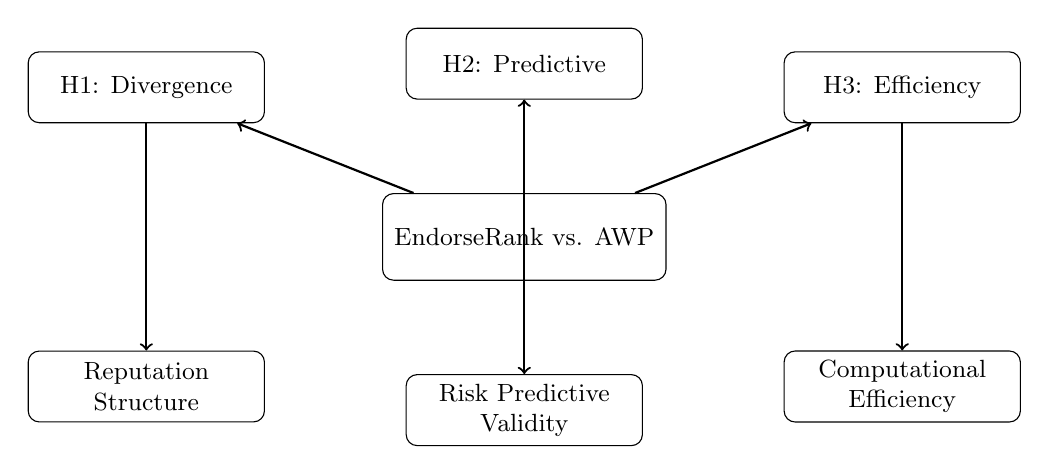
\begin{tikzpicture}[
  font=\small,
  box/.style={draw, rounded corners, align=center, minimum width=3.6cm, minimum height=1.1cm},
  smallbox/.style={draw, rounded corners, align=center, minimum width=3.0cm, minimum height=0.9cm},
  arrow/.style={->, thick}
]
\node[box] (center) at (0,0) {EndorseRank vs. AWP};
\node[smallbox] (h1) at (-4.8,1.9) {H1: Divergence};
\node[smallbox] (rep) at (-4.8,-1.9) {Reputation\\Structure};
\node[smallbox] (h2) at (0,2.2) {H2: Predictive};
\node[smallbox] (risk) at (0,-2.2) {Risk Predictive\\Validity};
\node[smallbox] (h3) at (4.8,1.9) {H3: Efficiency};
\node[smallbox] (eff) at (4.8,-1.9) {Computational\\Efficiency};
\draw[arrow] (center) -- (h1);
\draw[arrow] (center) -- (h2);
\draw[arrow] (center) -- (h3);
\draw[arrow] (h1) -- (rep);
\draw[arrow] (h2) -- (risk);
\draw[arrow] (h3) -- (eff);
\end{tikzpicture}

\end{center}


\begin{center}Figure 1: EndorseRank vs. AWP: hypotheses and evaluation constructs\end{center}

\textbf{H1 (Divergence): }EndorseRank and AWP will yield significantly different wallet orderings, demonstrating that an approve/permit--based endorsement graph creates a distinct reputation structure.


\textbf{H2 (Predictive Validity): }EndorseRank's scores will correlate more strongly with actual default events than AWP's scores, indicating superior predictive power.


\textbf{H3 (Computational Efficiency): }EndorseRank will require less runtime, memory, and fewer iterations to converge than AWP, demonstrating practical scalability advantages.


\phantomsection
\subsection*{4.3 Theoretical Justification}
\label{sec:theoretical-justification}
\addcontentsline{toc}{subsection}{4.3 Theoretical Justification}

\textbf{Hyperlink--Citation Semantics: }The original PageRank algorithm (Page et al., 1998) evaluates a webpage's importance by the structure of inbound hyperlinks, treating each link like a citation in an academic paper: pages that are linked to by many important pages receive higher rank. ERC- 20 approve/permit edges can be interpreted similarly, where an approval from wallet A to wallet B functions as a trust citation, justifying the use of PageRank on an approval graph.


\textbf{Predictive Validity Framework: }In credit scoring and psychometrics, predictive validity assesses how well a metric forecasts real-world outcomes.


By treating EndorseRank and AWP scores as assessment scales, we employ standard metrics (AUC, Precision, Recall, F1-score) to compare their ability to predict defaults.


\textbf{Computational Complexity Theory: }PageRank's time complexity per iteration is O(---E---). Approve/permit graphs are sparser than transfer- based graphs (fewer edges ---E---), leading to lower per-iteration cost, faster convergence, and reduced memory usage.


\phantomsection
\subsection*{4.4 Implications for Research Design}
\label{sec:implications-for-research-design}
\addcontentsline{toc}{subsection}{4.4 Implications for Research Design}

\textbf{Measurement: }Compute EndorseRank and AWP scores for a matched sample of Aave wallets, record default outcomes over a defined period, and profile each algorithm's runtime, memory usage, and iterations to convergence.


\proposalSubheading{Analysis:}

\textbf{H1 }via rank correlation (Spearman's \emph{\(\rho\)}, Kendall's \emph{\(\tau\)})


\textbf{H2 }via predictive metrics (AUC, Precision, Recall, F1-score)


\textbf{H3 }via paired benchmarks of runtime, peak memory, and iteration counts


\textbf{Contribution: }By anchoring our hypotheses in established theories, this framework ensures that empirical results will offer both scholarly rigor and practical relevance, demonstrating EndorseRank's advantages in producing a semantically meaningful, predictive, and efficient on-chain reputation metric.


\clearpage
\phantomsection
\section*{5 \textbf{Research Methodology}}
\label{sec:research-methodology}
\addcontentsline{toc}{section}{5 Research Methodology}

This section outlines the overall approach for implementing EndorseRank, comparing it to Adaptive Weighted PageRank (AWP), and evaluating their performance in terms of reputation structure, predictive validity, and computational efficiency.


\phantomsection
\subsection*{5.1 Research Design and Method}
\label{sec:research-design-and-method}
\addcontentsline{toc}{subsection}{5.1 Research Design and Method}

\textbf{Dataset Overview}


This study uses public, on-chain event logs as the primary dataset. The raw data are time-stamped, address-level records emitted by Ethereum smart contracts, which makes them reproducible but also inherently pseudonymous (wallets are identifiers, not verified real-world entities).


\textbf{Core unit of analysis}


Wallet addresses and directed relationships between wallets (owner \(\to\) spender), later represented as a sparse graph.


\textbf{Primary signals}


ERC-20 Approve (and EIP-2612 Permit) authorizations that specify an owner, a spender, and an allowance amount (with token contracts providing the context for each authorization).


\textbf{Sparsity and heavy tails}


Endorsement/authorization graphs are expected to be highly sparse with skewed degree/weight distributions (a small number of contracts/routers receive many approvals), which motivates robust evaluation beyond mean-based summaries.


\textbf{Temporal structure}


Events form a time series; we operationalize EndorseRank on a fixed observation window and construct ``latest state'' edge weights by retaining the most recent relevant allowance information per relationship.


\textbf{Data quality consideration}s


Event logs are generally reliable but can include revocations (amount = 0), ``spend-all by default'' approvals, and occasional indexing gaps; these characteristics are treated explicitly in preprocessing and robustness checks.


Data Collection \& Preprocessing


\textbf{Blockchain Data Source}


Ethereum mainnet (January 1, 2025 -- June 30, 2025) via Google BigQuery or an archive node.


Event Extraction


Approval/permit-derived authorizations: all ERC-20 Approval(owner, spender, value) events, including approvals generated through permit-compatible flows where the token emits the standard Approval event; where permit-specific traces are available, they will be used only to validate the authorization source.


Default Labels


Aave V3 liquidation events will be used as the observable on-chain proxy for default. A wallet will be labelled as defaulted only when the liquidation outcome occurs after the feature-observation window, so that EndorseRank and baseline scores are computed before the outcome they are used to predict.


Sampling


Sampling: the predictive analysis will use the full set of Aave V3-active wallets that appear in the observation window and have sufficient event history for feature construction. Computational benchmarks will use a reproducible random sample of 100,000 wallets with a fixed seed, and robustness checks will compare 50,000- and 200,000-wallet samples to test scalability sensitivity.


\begin{longtable}{>{\raggedright\arraybackslash}p{0.18\linewidth}>{\raggedright\arraybackslash}p{0.39\linewidth}>{\raggedright\arraybackslash}p{0.35\linewidth}}
\toprule
\textbf{Construct} & \textbf{Definition} & \textbf{Associated Variables} \\
\midrule
Reputation\newline Structure & The pattern and relative ordering\newline of wallet reputations produced by\newline a ranking algorithm. & (1) EndorseRank score;\newline AWP score;\newline Rank correlation(Spear- man's \emph{\(\rho\) }/ Kendall's \emph{\(\tau\) }) between EndorseRank and AWP \\
\addlinespace
Risk Predictive\newline Validity & The extent to which a reputation score forecasts actual default events on a DeFi platform. & Default status (binary);\newline EndorseRank's predictive metrics (AUC, Precision/Recall, F1- score);\newline AWP's predictive metrics \\
\addlinespace
Computational\newline Efficiency & The computational resources(time, memory, convergence iterations) required to compute\newline scores. & (7) EndorseRank runtime;\newline AWP runtime;\newline Peak memory usage;\newline Iterations to convergence \\
\addlinespace
\bottomrule
\end{longtable}

\proposalSubheading{1. Graph Construction \& Algorithm Implementation}

\begin{itemize}
\item[\textbullet] \textbf{Approve/Permit Graph }($G_{\text{approve}}$)
\begin{itemize}
\item[\textendash] \textbf{Nodes}: Wallet addresses.
\item[\textendash] Edges: directed owner-to-spender relationships weighted by the latest nonzero allowance from u to v. Because ERC-20 tokens differ in decimals and economic scale, weights will first be token-decimal adjusted; sensitivity checks will compare raw allowance weights, log-transformed weights, and value-normalized weights where reliable price data are available.
\end{itemize}
\item[\textbullet] \textbf{Transfer-Based Graph }($G_{\text{transfer}}$)
\begin{itemize}
\item[\textendash] Same node set; edges weighted by sum of transfer amounts \emph{u }\(\to\) \emph{v}.
\end{itemize}
\item[\textbullet] Algorithms
\end{itemize}
\textbf{EndorseRank: Weighted PageRank on }$G_{\text{approve}}$\textbf{with damping factor d = 0.85. This value is retained because 0.85 is the standard PageRank setting, provides a stable balance between diffusion and teleportation, and enables direct comparison with prior graph-ranking studies.}


\begin{itemize}
\item[\textendash] \textbf{AWP Reproduction}: Adaptive Weighted PageRank on $G_{\text{transfer}}$
\end{itemize}
incorporating time and value decay per Do et al. (2023).


\begin{itemize}
\item[\textbullet] Tools \& Environment
\begin{itemize}
\item[\textendash] Python with NetworkX or GraphFrames; Scipy sparse solvers; Docker containers for reproducibility.
\end{itemize}
\end{itemize}
\proposalSubheading{2. Performance Evaluation Procedures}

\begin{itemize}
\item[\textbullet] Predictive Performance
\begin{itemize}
\item[\textendash] Features: EndorseRank and AWP scores.
\item[\textendash] Labels: Binary default status.
\item[\textendash] Models: Logistic regression and random forest. Logistic regression is used as an interpretable linear baseline, while random forest captures nonlinear interactions and offers a stronger benchmark for mixed on-chain feature patterns.
\item[\textendash] Metrics: AUC, Precision@k, Recall, F1-score.
\end{itemize}
\item[\textbullet] Validation: 5-fold cross-validation, reporting mean +/- SD. Five folds provide a practical bias-variance trade-off while keeping repeated model fitting manageable for multiple baselines, robustness checks, and hardware-limited experiments.
\begin{itemize}
\item[\textendash] Temporal validation will be used alongside cross-validation to prevent look-ahead bias: graph features and reputation scores will be computed from events before the prediction cut-off, while liquidation/default labels will be drawn from a subsequent outcome window. This separation ensures that the model is evaluated on forward-looking predictive performance rather than on information that would not have been available at scoring time.
\end{itemize}
\item[\textbullet] Rank Divergence
\begin{itemize}
\item[\textendash] Compute Spearman's \emph{\(\rho\) }and Kendall's \emph{\(\tau\) }between EndorseRank and AWP.
\item[\textendash] Visualize via scatter plots and top-k Jaccard overlap.
\end{itemize}
\item[\textbullet] Computational Efficiency
\begin{itemize}
\item[\textendash] Hardware: Fixed 22-vCPU, 64 GB RAM server.
\item[\textendash] Measures:
\end{itemize}
\end{itemize}
\(\ast\) Runtime (graph build + PageRank convergence, averaged over 5 runs)


\(\ast\) Peak memory usage


\(\ast\) Iterations to reach tolerance 10\textsuperscript{-}\textsuperscript{6}


\phantomsection
\subsection*{5.1 Data Analysis}
\label{sec:data-analysis}
\addcontentsline{toc}{subsection}{5.1 Data Analysis}

\proposalSubheading{1. Hypothesis Testing}

\begin{itemize}
\item[\textbullet] \textbf{H1 (Divergence)}
\begin{itemize}
\item[\textendash] Test whether rank correlations differ significantly from 1 using a one- sample t-test or Wilcoxon signed-rank test.
\end{itemize}
\item[\textbullet] H2 (Predictive Validity)
\begin{itemize}
\item[\textendash] Compare AUCs via DeLong's test for correlated ROC curves.
\item[\textendash] Compare Precision, Recall, F1-scores via paired bootstrap confidence intervals.
\end{itemize}
\item[\textbullet] H3 (Computational Efficiency)
\begin{itemize}
\item[\textendash] Paired t-tests (or Wilcoxon tests if non-normal) on runtime, memory, and iteration counts.
\end{itemize}
\end{itemize}
\proposalSubheading{2. Robustness Checks}

\begin{itemize}
\item[\textbullet] Vary damping factor \emph{d }\(\in\) \{0\emph{.}75\emph{, }0\emph{.}85\emph{, }0\emph{.}95\}.
\item[\textbullet] Repeat analyses on subgraphs of top ERC-20 tokens by volume.
\item[\textbullet] Assess sensitivity to sample size (50k vs. 200k wallets).
\end{itemize}
\proposalSubheading{3. Reproducibility}

\begin{itemize}
\item[\textbullet] All code, queries, and analysis scripts versioned on GitHub.
\item[\textbullet] Data snapshots and Docker images preserved for full replication of results.
\end{itemize}
This methodological framework ensures a rigorous, reproducible evaluation of EndorseRank's advantages over existing PageRank-based approaches in reputation structure, risk prediction, and computational performance.


\clearpage
\phantomsection
\section*{6 \textbf{Limitations}}
\label{sec:limitations}
\addcontentsline{toc}{section}{6 Limitations}

While this study is designed to rigorously evaluate EndorseRank against Adaptive Weighted PageRank, we acknowledge several inherent limitations and potential threats to validity:


\proposalSubheading{1. Data Coverage and Quality}

\begin{itemize}
\item[\textbullet] \textbf{Event Completeness: We rely on public event logs (Approve, Permit, Transfer) from Ethereum archives or BigQuery. Some missing or misindexed events (e.g., due to chain reorganizations or node sync issues) may bias graph construction.}
\item[\textbullet] \textbf{Label Noise}: Default labels are derived from Aave V3 liquidation events; wallets that become underwater without on-chain liquidation (e.g., off- chain settlements) will be misclassified.
\end{itemize}
\proposalSubheading{2. Temporal Scope}

\begin{itemize}
\item[\textbullet] \textbf{Fixed Window}: Limiting analysis to a single six-month window may not capture longer-term reputation dynamics or market regime shifts. Results may differ for other periods, especially during high volatility or protocol upgrades.
\end{itemize}
\proposalSubheading{3. Graph Modeling Assumptions}

\begin{itemize}
\item[\textbullet] \textbf{Approval Semantics}: We assume that any nonzero approve/permit rep- resents a substantive trust endorsement. In practice, users may issue
\end{itemize}
``spend-all'' approvals by default or interact via custodial services, which dilute the trust signal.


\begin{itemize}
\item[\textbullet] \textbf{Edge Weight Aggregation}: Summing all transfers or using only the latest allowance ignores the provenance of funds and may obscure multi- token or multi-chain interactions.
\end{itemize}
\proposalSubheading{4. Algorithmic Simplifications}

\begin{itemize}
\item[\textbullet] \textbf{Fixed Damping Factor}: We apply a single damping factor (d = 0.85) uniformly; in reality, the optimal factor may vary by token, wallet type, or network segment.
\item[\textbullet] \textbf{Unmodeled Attributes}: EndorseRank ignores off-chain factors (e.g., KYC status, IP geolocation) and non-ERC-20 relationships (e.g., NFT approvals, cross-chain bridges), which may also influence trust.
\end{itemize}
\proposalSubheading{5. Generalizability}

\begin{itemize}
\item[\textbullet] \textbf{Protocol Specificity}: We focus on Aave V3 for default labels. EndorseRank's predictive power may differ for other lending protocols (Compound, MakerDAO) or non-lending use cases.
\item[\textbullet] \textbf{Asset Bias}: High-volume tokens (e.g., USDC, WETH) dominate graph structure; smaller or emerging tokens may yield sparse endorsement net- works less amenable to PageRank.
\end{itemize}
\proposalSubheading{6. Adversarial Manipulation and Sybil Attacks}

\begin{itemize}
\item[\textbullet] \textbf{Gaming the Graph}: Malicious actors could issue dummy approvals or orchestrate circular allowance patterns to inflate their EndorseRank score. Detecting and mitigating such Sybil strategies require additional safe- guards beyond the scope of this study.
\end{itemize}
\proposalSubheading{7. Computational Constraints}

\begin{itemize}
\item[\textbullet] \textbf{Scalability Limitations}: Although EndorseRank is more efficient than AWP on our sample, real-time computation on the full Ethereum graph
\end{itemize}
(millions of wallets) may still demand distributed computing or approximation techniques.


\clearpage
\phantomsection
\section*{7 \textbf{Ethics Considerations}}
\label{sec:ethics-considerations}
\addcontentsline{toc}{section}{7 Ethics Considerations}

Although this research relies exclusively on publicly available blockchain data, we will observe the following ethical principles to ensure responsible conduct. Because the study uses non-personal, public ledger data and does not intervene with human participants, it will align with UNISA's research ethics principles on privacy, confidentiality, responsible data management, and prior ethics reviews where required.


Ethics clearance process: before starting the empirical data collection and analysis phase, the researcher will submit the proposal, data-management plan, and public-data justification to the relevant UNISA School ethics process. If the study is classified as exempt or low risk because it uses public pseudonymous blockchain data and no human-participant intervention, the exemption or clearance confirmation will be retained as part of the research record. No attempt will be made to deanonymize wallet owners, combine wallet addresses with off-chain personal data, or publish address-level findings in a way that could reasonably identify individuals.


\proposalSubheading{1. Privacy and Anonymity}

\begin{itemize}
\item[\textbullet] \textbf{Pseudonymity Respect}: Ethereum addresses are pseudonymous, not inherently linked to real-world identities. We will not attempt to deanonymize addresses or correlate them with personally identifying information.
\item[\textbullet] \textbf{No Sensitive Data Collection}: We will restrict data collection to on- chain events (approve, permit, transfer, liquidation) and avoid scraping or integrating off-chain data such as IP addresses or KYC records.
\end{itemize}
\proposalSubheading{2. Data Usage and Compliance}

\begin{itemize}
\item[\textbullet] \textbf{Open Data Sources}: All queries will target public datasets (e.g., Google BigQuery, The Graph) in accordance with their terms of service and rate limits.
\item[\textbullet] \textbf{No Malicious Interaction}: We will not broadcast transactions or otherwise interact with smart contracts in ways that could disrupt network operations or degrade performance.
\end{itemize}
\proposalSubheading{3. Fairness and Bias Mitigation}

\begin{itemize}
\item[\textbullet] \textbf{Algorithmic Fairness}: We will audit EndorseRank and AWP for un- intended biases---e.g., systematically undervaluing new entrants or low- volume participants---and discuss these limitations in our analysis.
\item[\textbullet] \textbf{Transparency}: All code, parameter choices, and evaluation metrics will be documented and published, enabling peer review and independent replication.
\end{itemize}
\proposalSubheading{4. Responsible Disclosure}

\begin{itemize}
\item[\textbullet] \textbf{Vulnerability Reporting}: If our analysis uncovers potential vulnerabilities in smart contracts (e.g., unexpected approval patterns that could be exploited), we will confidentially notify the responsible protocol teams before public disclosure.
\end{itemize}
\proposalSubheading{5. Social and Financial Impact}

\begin{itemize}
\item[\textbullet] \textbf{No Financial Advice}: Although EndorseRank may inform risk assessment, we will explicitly disclaim that it is not financial advice and highlight the need for human oversight in lending decisions.
\item[\textbullet] \textbf{Avoiding Misuse}: We will discuss potential adversarial manipulation (e.g., Sybil attacks) and recommend safeguards so that our methodology is not misused to target or disadvantage specific users.
\end{itemize}
By adhering to these practices, we ensure that our research advances on-chain reputation modeling ethically, respects user privacy, and contributes responsibly to the DeFi ecosystem.


\clearpage
\phantomsection
\section*{8 \textbf{Significance of Research}}
\label{sec:significance-of-research}
\addcontentsline{toc}{section}{8 Significance of Research}

This research advances the field of on-chain reputation scoring and decentralized credit assessment in several meaningful ways. At the doctoral level, the intended original contribution is the formulation and empirical validation of allowance-based wallet reputation as a distinct class of on-chain trust signal. The study is positioned to contribute new knowledge by showing whether explicit authorization relationships can produce a reputation metric that is theoretically interpretable, predictive of financial risk, and computationally more scalable than transaction-history-based PageRank baselines:


\proposalSubheading{1. Theoretical Innovation}

\begin{itemize}
\item[\textbullet] \textbf{Endorsement-Based Graph Modeling}: By introducing a directed, weighted endorsement graph derived from ERC-20 approve and permit events, EndorseRank extends the original PageRank citation paradigm to capture explicit on-chain trust signals. This conceptual shift---from token transfers to authorization links---broadens the theoretical underpinnings of network centrality in blockchain contexts.
\item[\textbullet] \textbf{Temporal Simplification}: Unlike existing approaches that require elaborate time-decay functions, EndorseRank leverages the override semantics of ERC-20 allowances to dispense with time-based weighting, offering a cleaner, more principled framework for modeling enduring trust relationships.
\end{itemize}
\proposalSubheading{2. Methodological Contribution}

\begin{itemize}
\item[\textbullet] \textbf{Efficient Computation}: EndorseRank demonstrates that a sparser approval graph can yield reputation scores with comparable or superior predictive power to transfer-based PageRank, while reducing computation time, memory usage, and convergence iterations. This efficiency gain makes large-scale, near-real-time reputation scoring more feasible for resource-constrained DeFi platforms.
\item[\textbullet] \textbf{Reproducible Framework}: We provide a fully specified, open-source pipeline---from blockchain data extraction to PageRank implementation and evaluation metrics---enabling other researchers and practitioners to validate, extend, and apply the EndorseRank methodology across different protocols and ecosystems.
\end{itemize}
\proposalSubheading{3. Practical Impact}

\begin{itemize}
\item[\textbullet] \textbf{Improved Risk Management}: By more accurately identifying wallets at risk of default, EndorseRank can help lenders reduce collateral requirements for trustworthy users, paving the way for under-collateralized and more inclusive lending products. This has the potential to unlock significant liquidity in DeFi and broaden access to financial services.
\item[\textbullet] \textbf{Protocol Integration}: The lightweight nature of EndorseRank makes it a strong candidate for integration into on-chain or off-chain risk oracles, governance dashboards, and compliance tools, providing actionable intelligence to DeFi protocols, custodial services, and regulators.
\end{itemize}
\proposalSubheading{4. Broader Implications}

\begin{itemize}
\item[\textbullet] \textbf{Cross-Protocol Applicability}: While this study focuses on Ethereum and Aave, the EndorseRank approach generalizes to any ERC-20--compatible network or custom token standard, making it relevant for emerging L2 solutions and alternative smart-contract platforms.
\item[\textbullet] \textbf{Foundation for Future Research}: By highlighting the value of authorization networks, this work encourages further exploration of other on-chain signals---such as governance votes, staking approvals, and cross- chain bridges---and their integration into composite reputation and identity frameworks.
\end{itemize}
\clearpage
\phantomsection
\section*{9 \textbf{Schedule}}
\label{sec:schedule}
\addcontentsline{toc}{section}{9 Schedule}

The following 20-month schedule assumes that the research proposal will be approved by 31 May 2026. The revised timeline therefore begins with post-approval research activities in June 2026 and includes thesis-writing milestones as well as the preparation and submission of journal articles based on the research results.


\begin{longtable}{>{\raggedright\arraybackslash}p{0.18\linewidth}>{\raggedright\arraybackslash}p{0.39\linewidth}>{\raggedright\arraybackslash}p{0.35\linewidth}}
\caption{Research Project Schedule}\\
\toprule
\textbf{Period} & \textbf{Activities} & \textbf{Deliverables} \\
\midrule
By 31 May 2026 & Complete final proposal revisions\newline Obtain supervisor and departmental approval of the proposal\newline Confirm the approved research scope and timeline & Approved research proposal\newline Confirmed post-approval work plan \\
\addlinespace
June 2026 & Prepare the post-approval research protocol\newline Finalize data-management and ethics-alignment procedures\newline Set up the development and analysis environment & Approved research protocol\newline Data-management checklist\newline Configured research environment \\
\addlinespace
July-Aug 2026 & Develop and test the data-acquisition pipeline\newline Extract ERC-20 Approve/Permit and Transfer events\\Identify and label Aave liquidation transactions & ETL scripts\newline Raw event datasets\newline Liquidation labels file \\
\addlinespace
Sep-Oct 2026 & Clean and validate the extracted datasets\newline Construct wallet-transaction graphs\newline Engineer allowance, transfer, and liquidation-related features & Validated analysis dataset\newline Wallet graph datasets\newline Feature dictionary \\
\addlinespace
Nov-Dec 2026 & Implement the EndorseRank reputation-scoring model\newline Implement AWP and PageRank baselines\newline Run initial parameter-sensitivity checks & Model implementation\newline Baseline implementation\newline Preliminary scoring outputs \\
\addlinespace
Jan-Feb 2027 & Evaluate rank correlation and predictive validity\newline Run logistic regression and random forest experiments\newline Assess computational efficiency and robustness & Evaluation results\newline Risk-prediction results\newline Robustness and efficiency analysis \\
\addlinespace
March 2027 & Interpret empirical results\newline Prepare figures, tables, and chapter-level findings\newline Discuss results against the research objectives & Results chapter materials\newline Updated analysis tables and figures \\
\addlinespace
April 2027 & Draft the first journal article from the model and evaluation results\newline Align the article with an accredited journal scope\newline Circulate the draft for supervisor feedback & First journal article draft\newline Target journal shortlist\newline Supervisor feedback record \\
\addlinespace
May 2027 & Revise and submit the first journal article to an accredited journal\newline Incorporate article findings into the thesis draft & Submitted first journal article\newline Updated thesis results chapter \\
\addlinespace
June-July 2027 & Draft and revise the introduction, literature review, and methodology chapters\newline Integrate supervisor comments across completed chapters\newline Check consistency between objectives, methods, and results & Revised thesis chapters\newline Integrated supervisor feedback \\
\addlinespace
August 2027 & Draft the second publication from the DeFi reputation and risk-scoring findings\newline Position the contribution against related work\newline Prepare publication tables and supporting evidence & Second publication draft\newline Publication-ready tables and evidence \\
\addlinespace
September 2027 & Revise and submit the second article to an accredited journal\newline Update the thesis discussion with publication feedback where applicable & Submitted second journal article\newline Updated discussion chapter \\
\addlinespace
October 2027 & Complete the full thesis draft\newline Finalize conclusions, limitations, and future-work sections\newline Conduct internal consistency and reference checks & Complete thesis draft\newline Checked references and cross-references \\
\addlinespace
November-December 2027 & Revise the full thesis based on supervisor feedback\newline Edit formatting, language, tables, and figures\newline Prepare submission documentation & Final revised thesis\newline Submission-ready document\newline Completed administrative documents \\
\addlinespace
January 2028 & Obtain final supervisor sign-off\newline Submit the thesis for examination\newline Track journal-review outcomes and respond to editorial queries if required & Submitted thesis\newline Supervisor sign-off\newline Journal response plan \\
\addlinespace
\bottomrule
\end{longtable}

\clearpage
\phantomsection
\section*{10 \textbf{Dissertation/Thesis Outline}}
\label{sec:dissertationthesis-outline}
\addcontentsline{toc}{section}{10 Dissertation/Thesis Outline}

The Dissertation consists of the following six chapters:


\begin{itemize}
\item[\textendash] Chapter 1: Introduction and research problem. This chapter will refine the proposal into the thesis introduction by presenting the DeFi lending context, the on-chain wallet reputation problem, the research questions, objectives, scope, significance, and limitations.
\item[\textendash] Chapter 2: Literature review and theoretical framework. This chapter will expand the proposal literature review into a comprehensive analysis of graph-based reputation scoring, DeFi credit-risk prediction, ERC-20 allowance semantics, PageRank variants, and theoretical foundations for reputation structure, predictive validity, and computational efficiency.
\item[\textendash] Chapter 3: Research methodology. This chapter will specify the philosophical position, research design, data sources, sampling logic, feature engineering, graph-construction procedures, baseline reproduction, statistical tests, robustness checks, ethics clearance, and reproducibility controls.
\item[\textendash] Chapter 4: Implementation and empirical results. This chapter will report on the data pipeline, EndorseRank implementation, baseline implementations, dataset characteristics, graph statistics, predictive-model results, rank-divergence findings, and computational benchmark outcomes.
\item[\textendash] Chapter 5: Discussion. This chapter will interpret the findings against each research question and objective, explain the theoretical and practical implications for DeFi risk assessment, evaluate threats to validity, and discuss how the results support or limit the claimed contribution.
\item[\textendash] Chapter 6: Conclusion and future work. This chapter will synthesize the study, state the original contribution to knowledge, revisit the research questions, summarize limitations, and propose future work on cross-protocol validation, adversarial manipulation, and broader on-chain trust signals.
\end{itemize}
\phantomsection
\subsection*{9.1 References}
\label{sec:references}
\addcontentsline{toc}{subsection}{9.1 References}

\hangindent=0.5in \hangafter=1 3Jane Protocol. (n.d.). Jane Score documentation.\par

\hangindent=0.5in \hangafter=1 Blockchain Bureau. (n.d.). Providence score documentation.\par

\hangindent=0.5in \hangafter=1 Cred Protocol. (n.d.). Cred Score documentation.\par

\hangindent=0.5in \hangafter=1 Do, H. D., et al. (2023). PageRank and HodgeRank on Ethereum transactions: A measure for social credit. International Journal of Software Innovation, 11(1).\par

\hangindent=0.5in \hangafter=1 Ethereum Improvement Proposals. (2015). ERC-20 token standard (EIP-20). \href{https://eips.ethereum.org/EIPS/eip-20}{https://eips.ethereum.org/EIPS/eip-20}\par

\hangindent=0.5in \hangafter=1 Ethereum Improvement Proposals. (2020). ERC-20 permit extension (EIP-2612). \href{https://eips.ethereum.org/EIPS/eip-2612}{https://eips.ethereum.org/EIPS/eip-2612}\par

\hangindent=0.5in \hangafter=1 Ghosh, R., et al. (2024). On-chain credit risk score in decentralized finance. arXiv. \href{https://arxiv.org/abs/2412.00710}{https://arxiv.org/abs/2412.00710}\par

\hangindent=0.5in \hangafter=1 Hassija, V., et al. (2020). Secure lending: Blockchain and prospect theory-based decentralized credit scoring model. IEEE Transactions on Network Science and Engineering, 7(4).\par

\hangindent=0.5in \hangafter=1 Imig, S. (2023). Trustworthiness and PageRank on the Ethereum blockchain. SSRN.\par

\hangindent=0.5in \hangafter=1 Jain, D., et al. (2019). Bit-Score: A blockchain-based distributed network for secure credit scoring. In Proceedings of ICCCA.\par

\hangindent=0.5in \hangafter=1 Page, L., Brin, S., Motwani, R., \& Winograd, T. (1998). The PageRank citation ranking: Bringing order to the web. Stanford Digital Library Technologies Project.\par

\hangindent=0.5in \hangafter=1 Wolf, W., et al. (2022). Scoring Aave accounts for creditworthiness. arXiv. https://arxiv.org/abs/2207.07008\par

\hangindent=0.5in \hangafter=1 Yang, F., et al. (2024). RiskProp: Account risk rating on Ethereum via de-anonymous score and network propagation. IEEE Transactions on Dependable and Secure Computing.\par

\clearpage
\phantomsection
\section*{11 \textbf{Appendices}}
\label{sec:appendices}
\addcontentsline{toc}{section}{11 Appendices}

None.


\end{document}